\documentclass{article}

\usepackage{graphicx}
\usepackage{tikz}
\usepackage{tikzsymbols}
\usetikzlibrary{calc,patterns,shapes.geometric}
\pagestyle{empty}
\usepackage[margin=0pt]{geometry}
\geometry{papersize={14in,12in}}

\def\centerarc[#1](#2)(#3:#4:#5){\draw[#1] ($(#2)+({#5*cos(#3)},{#5*sin(#3)})$) arc (#3:#4:#5);}

\begin{document}
	\begin{figure}
		\centering
		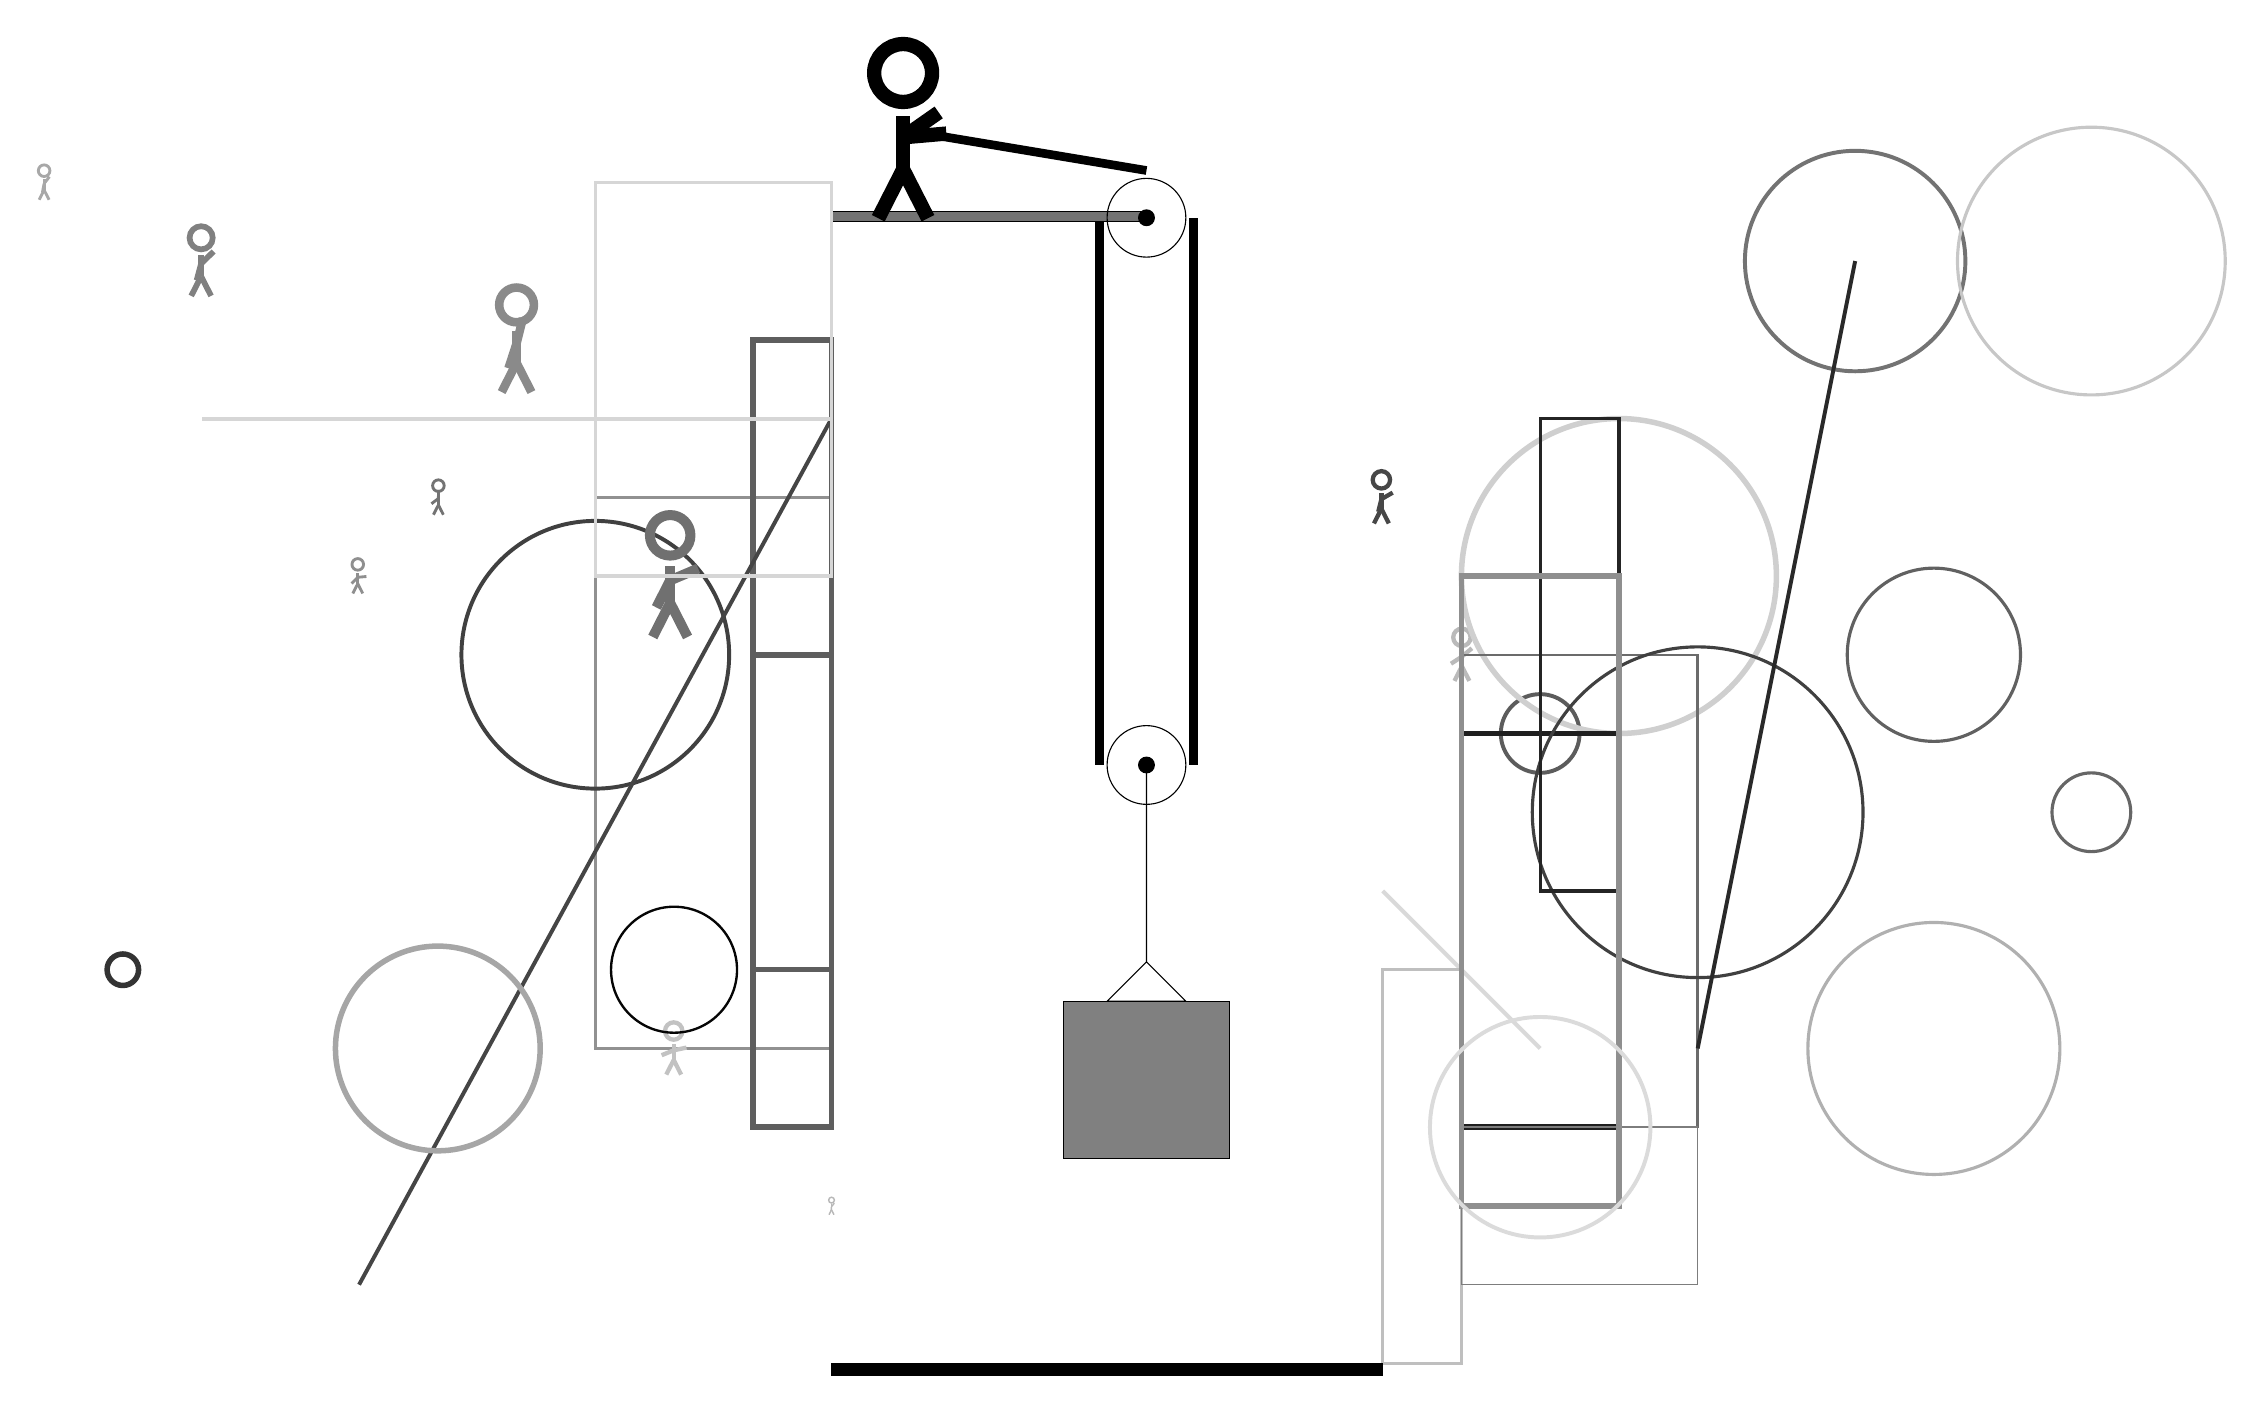
\begin{tikzpicture}
			%%%%% START %%%%%
			
			\draw[fill=black!55] (-2, 11.5) rectangle (2, 11.625);
			
			\draw (2, 4.6) circle (0.5);
			\draw[fill=black] (2, 4.6) circle (0.1);
			
			\draw (2, 11.55) circle (0.5);
			\draw[fill=black] (2, 11.55) circle (0.1);
			
			\draw [line width=0.5mm, color=black!55](11, 11) circle (1.4);
			
			\node[line width=0.3mm, color=black!27] at (6, 6) {\Strichmaxerl[3][33][40]};
			\draw[line width=0.4mm, color=black!43] (-2, 8) rectangle (-5, 1);
			\node[line width=0.7mm, color=black!28] at (-2, -1) {\Strichmaxerl[1][85][50]};
			\draw [line width=0.5mm, color=black!64](7, 5) circle (0.5);
			
			\draw [line width=0.7mm, color=black!19](8, 7) circle (2.0);
			\node[line width=0.5mm, color=black!72] at (5, 8) {\Strichmaxerl[3][76][30]};
			\node[line width=0.3mm, color=black!50] at (-10, 11) {\Strichmaxerl[4][75][44]};
			\draw[line width=0.7mm, color=black!88] (6, 5) rectangle (8, 0);
			\draw[line width=0.5mm, color=black!15](7, 1) -- (5, 3);
			\draw[line width=0.3mm, color=black!58] (6, 6) rectangle (9, 0);
			\draw [line width=0.4mm, color=black!75](9, 4) circle (2.1);
			\node[line width=0.2mm, color=black!44] at (-8, 7) {\Strichmaxerl[2][46][5]};
			
			\node[line width=0.7mm, color=black!34] at (-12, 12) {\Strichmaxerl[2][79][52]};
			\draw [line width=0.5mm, color=black!75](-5, 6) circle (1.7);
			\node[line width=0.2mm, color=black!56] at (-4, 7) {\Strichmaxerl[7][63][23]};
			
			\draw[line width=0.7mm, color=black!63] (-3, 10) rectangle (-2, 2);
			
			\draw[line width=0.5mm, color=black!73](-2, 9) -- (-8, -2);
			\draw[line width=0.5mm, color=black!84](9, 1) -- (11, 11);
			\draw [line width=0.4mm, color=black!31](12, 1) circle (1.6);
			\draw [line width=0.4mm, color=black!62](12, 6) circle (1.1);
			
			\draw [line width=0.7mm, color=black!35](-7, 1) circle (1.3);
			\draw[line width=0.4mm, color=black!25] (6, -3) rectangle (5, 2);
			\draw[line width=0.5mm, color=black!16](-2, 9) -- (-10, 9);
			\draw[line width=0.7mm, color=black!63] (-3, 6) rectangle (-2, 0);
			
			\node[line width=0.3mm, color=black!24] at (-4, 1) {\Strichmaxerl[3][22][12]};
			
			\node[line width=0.4mm, color=black!55] at (-7, 8) {\Strichmaxerl[2][37][89]};
			\draw [line width=0.7mm, color=black!80](-11, 2) circle (0.2);
			\draw [line width=0.4mm, color=black!60](14, 4) circle (0.5);
			\draw[line width=0.2mm, color=black!51] (6, -2) rectangle (9, 0);
			\node[line width=0.2mm, color=black!46] at (-6, 10) {\Strichmaxerl[6][72][76]};
			\draw[line width=0.4mm, color=black!86] (7, 3) rectangle (8, 9);
			\draw[line width=0.4mm, color=black!16] (-2, 12) rectangle (-5, 7);
			
			\draw [line width=0.4mm, color=black!22](14, 11) circle (1.7);
			\draw[line width=0.7mm, color=black!44] (6, -1) rectangle (8, 7);
			\draw [line width=0.3mm, color=black!98](-4, 2) circle (0.8);
			
			\draw [line width=0.5mm, color=black!14](7, 0) circle (1.4);
			
			\draw (2, 4.6) -- (2, 2.1) -- (1.5, 1.6) -- (2.5, 1.6) -- (2, 2.1);
			\draw[fill=black!50] (0.95, 1.6) rectangle (3.05, -0.4);
			
			\draw[line width=1.1mm] (1.4, 11.5) -- (1.4, 4.6);
			\centerarc[line width=1.1mm](2, 4.6)(180:360:0.6);
			\draw[line width=1.1mm](2.6, 4.6) -- (2.6, 11.55);
			\centerarc[line width=1.1mm](2, 11.55)(0:90:0.6);
			\draw[line width=1.1mm](2, 12.15) -- (-1, 12.65);
			
			\node at (-1, 12.65) {\Strichmaxerl[10][-175][35]};
			
			\draw[fill=black] (-2, -3) rectangle (5, -3.15);
			
			%%%%% END %%%%%
		\end{tikzpicture}
	\end{figure}	
\end{document}